\chapter{Safety and the PR2}
Point out which parts of the code are considered part of the hardware safety systems (e.g. joint current limits), and make it clear that changing them can cause problems.

Talk about guidelines for safe operation (e.g. is it OK in a normal lab environment?)

\chapter{PR2 hardware}

\section{What's in the box}
The PR2 will arrives in a big crate.  In the crate should be:
\subsection{PR2 robot}
\subsection{Wireless run-stop}
\label{wirelessrunstop}
The PR2 comes with an \href{http://www.omnexcontrols.com/products/portable/t50.html}{OMNEX T50} 
wireless run stop transmitter which when stopped or out of range will halt the motors and put the power system in standby mode. 

\begin{figure}[h]
\centering
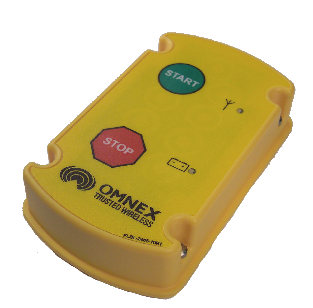
\includegraphics[width=150px]{run_stop.png}
\caption{The PR2 wireless run stop.}
\label{fig:runstop}
\end{figure}

To start the run stop transmitting, press the green start button (Figure~\ref{fig:runstop}) which will start the transmitting 
light flashing. While transmitting the run stop has a range of approximately 800ft. The run stop is powered by 4AA batteries 
when the batteries are low the battery light will flash warning you to change the batteries.

\subsection{Wireless Joystick}
The PR2 ships with a bluetooth joystick for teleoperating the robot. The bluetooth joystick is a 
\href{http://www.sonystyle.com/webapp/wcs/stores/servlet/ProductDisplay?catalogId=10551&storeId=10151&langId=-1&productId=8198552921665411965#additionalImage1%22}{Sony DUALSHOCK®3} 
wireless controller and can be charged using any standard USB A to mini-B USB cable. For more information please see the 
\href{http://www.ros.org/wiki/ps3joy}{ps3joy} package at \href{http://www.ros.org}{ros.org}.

\subsection{Base-station computer}
\section{Mechanism}
PR2 is a 32-dof mobile manipulator with a mobile base, two arms, and a variety of sensors on a pan-tilt head.
\subsection{Robot anatomy}
Include the information from the robot anatomy document here.  Official names of all components, links, and joints in the robot with pictures.
\subsection{Drivetrains}
Discuss the drive-train approach, how/why things work, what types of errors we expect to see and don't expect to see
\subsection{Motion control}
Describe motion control architecture, capabilities, performance.
\subsection{Mechanical specs}
\subsubsection{Environmental specs}
\subsubsection{Forces and torques}
\subsubsection{Joint limits and range of travel}

\section{Sensors}
The PR2 has a variety of sensors spread out over it's body:
\subsection{Base Laser}
The base laser of the PR2 is \href{http://www.hokuyo-aut.jp/02sensor/07scanner/utm_30lx.html}{Hokuyo Top-URG (UTM-30LX)} 
scanning range finder that has a 30m and 270$^\circ$ scanning range. For more information please see the 
\href{http://www.ros.org/wiki/hokuyo_node}{hokuyo\_node} package at \href{http://www.ros.org}{ros.org}.

\subsection{Tilting Laser}
In addition to the base laser, the PR2 has a \href{http://www.hokuyo-aut.jp/02sensor/07scanner/utm_30lx.html}{Hokuyo Top-URG (UTM-30LX)}
mounted on a tilting platform below the pan-tilt head. The tilting platform can sweep the scanning 
laser through 135$^\circ$ ($+90^\circ$ and $-45^\circ$ from level) and can be controlled using the
default laser\_tilt\_controller. For more information please see the \href{http://www.ros.org/wiki/hokuyo_node}{hokuyo\_node} 
and \href{http://www.ros.org/wiki/pr2_default_controllers}{pr2\_default\_controllers} packages at \href{http://www.ros.org}{ros.org}.

\subsection{Head Cameras}
The PR2 pan-tilt head has three cameras and a textured light projector:
\begin{description}

\item[Wide Stereo Camera]
The wide stereo of the PR2 is part of the dual stereo pair and is a 100Mb color ethernet camera. The wide stereo uses the
\href{http://www.aptina.com/products/image_sensors/mt9v032c12stc/#overview}{Aptina MT9V032C12STC} imager chip
and has a max resolution of 752 x 480 pixels at 15 fps. The camera has a field of view (FOV) of approximately 
$90^\circ$ and a 2.5mm F2.5 \href{http://www.mars-cam.com/lenses/ccd_cmos/Technology%20Report(V-4402.5-2.5-HR).pdf}{Marshall V-4402.5-2.5-HR} 
lens. For more information please see the \href{http://www.ros.org/wiki/wge100_camera}{TODO} package
at \href{http://www.ros.org}{ros.org}.

\item[Narrow Stereo Camera]
The narrow stereo of the PR2 is part of the dual stereo pair and is a 100Mb monchrome ethernet camera. 
The narrow stereo uses the \href{http://www.aptina.com/products/image_sensors/mt9v032c12stm/#overview}{Aptina MT9V032C12STM} 
imager chip and has a max resolution of 752 x 480 pixels at 15 fps. The camera has a FOV of approximately $55^\circ$ and 
a 5.6mm F2.0  \href{http://www.mars-cam.com/lenses/ccd_cmos/Technology%20Report(V-4405.6-2.0-HR).pdf}{Marshall V-4405.6-2.0-HR}
lens. For more information please see the \href{http://www.ros.org/wiki/wge100_camera}{TODO} package
at \href{http://www.ros.org}{ros.org}.

\item[Gigabit Ethernet Camera]
The PR2 has a gigabit ethernet camera located to the left of the dual stereo pair on the pan-tilt head. 
The gigabit ethernet camera is a \href{http://www.prosilica.com/products/gc2450.html}{Prosilica GC2450C} 
which uses the Sony ICX-625AQ imager chip and has a max resolution of 2448 x 2050 pixels at 15 fps. 
Additionally, the gigabit ethernet camera has a 8mm F1.4-F16 \href{http://www.kowascope.com/frontend/proddetail.asp?pn=LM8JC&co=10000348}{Kowa LM8JC} lens.
For more information please see the \href{http://www.ros.org/wiki/prosilica_camera}{prosilica\_camera} package
at \href{http://www.ros.org}{ros.org}.

\item[Textured Light Projector]
The PR2 has a textured light projector located to the right of the dual stereo pair on the pan-tilt head. The projector has a 
FOV of approximately $55^\circ$ and a 5.6mm F2.0 \href{http://www.kowascope.com/frontend/proddetail.asp?pn=LM12JC&co=10000348}{Kowa LM12JC} 
lens.  For more information please see the \href{http://www.ros.org/wiki/TODO}{TODO} package at \href{http://www.ros.org}{ros.org}.

\end{description}

\subsection{Forearm cameras}
Each forearm of the PR2 is equipped with a 12V 100Mb color ethernet camera. The forearm camera uses the 
\href{http://www.aptina.com/products/image_sensors/mt9v032c12stc/#overview}{Aptina MT9V032C12STC}  imager chip
and has a max resolution of 752 x 480 pixels at 15 fps. Additionally, the forearm camera has a 2.5mm F2.0 lens.  
For more information please see the \href{http://www.ros.org/wiki/wge100_camera}{wge100\_camera} package
at \href{http://www.ros.org}{ros.org}.

\subsection{Gripper Sensors}
\begin{description}

\item[Accelerometer]
The gripper of the PR2 is equipped with a \href{http://www.bosch-sensortec.com/content/language1/html/3474.htm}{Bosch BMA150} 
digital triaxal accelerometer. The measurement range ($\pm$2g, $\pm$4g, or $\pm$8g) and bandwidth (25Hz - 1500Hz) 
of the accelerometer can be selected in software. For more information please see the \href{http://www.ros.org/wiki/wge100_camera}{TODO} 
package at \href{http://www.ros.org}{ros.org}.

\item[Fingertip Pressure Sensors]


\item[Calibration LED]

\end{description}

\subsection{Inertial measurement unit}
The PR2 has an inertial measurement unit (IMU) located next to the tilting laser. The IMU is a 
\href{http://www.microstrain.com/3dm-gx2.aspx}{MicroStrain Inertial-Link 3DM-GX2} which has an 
accelerometer range of $\pm$5g and a gyro range of $300^\circ/s$. For more information please see 
the \href{http://www.ros.org/wiki/imu_node}{imu\_node} package at \href{http://www.ros.org}{ros.org}.

\subsection{Speaker}
The PR2 has two \href{http://www.logitech.com/index.cfm/speakers_audio/home_pc_speakers/devices/199&cl=us,en}{Logitech V20 notebook speakers} 
that are located under the pan-tilt head on either side of the tilting laser. For more information please 
see the \href{http://www.ros.org/wiki/sound_play}{sound\_play} package at \href{http://www.ros.org}{ros.org}.


\section{Power system}
\subsection{Overview}
The PR2 has a Lithium-ion (Li-ion) battery system that is charged off of 120V wall current and provides power the computers, motors, and sensors in the system.  Power distribution is controlled by the {\it Power Board}, which communicates over Ethernet.
\subsection{Power Busses}
The robot has several internal power busses:
\begin{description}
\item[120v] The robot has a 3-prong IEC320 plug in the back, which is connected through a circuit breaker to the inputs of the four AC-DC converters that are used to charge the battery packs.  The system is designed to pull up to 15A, so it is OK to plug the robot in to any 15A wall socket, but you should make sure there aren't other devices which draw significant power, such as computers, on the same circuit.
\item[Motor Power Bus] The motor controllers are fed from circuit breakers on the power board that can be in one of thre states.  When enabled, they provide a direct connection to the unregulated battery power, which ranges from 52V when the batteries are fully discharged up to 72V when connected to wall power.  When the motors are in standby mode, the power board provides a low-power 18V supply which is used for communication and to maintaing encoder position counts.  In the event of a major power-system problem, or if manually disabled, these circuit-breakers will also shut completely off without cutting power to the computers or sensors.  There are three independent motor power busses - left arm, right arm, and base/head.
\item[12V system bus]
12V power for sensors.  This is also the recommended source of power for user modifications. Provided by the power board.
\item[12V computer power]
12V power for computers.  Provided by the power board.
\subsection{Batteries}
The battery system has four battery bays comprised of four \href{http://www.oceanserver-store.com/18.html}{Ocean Server BA95HC-FL}
14.4V Li-ion batteries, a \href{http://www.v-infinity.com/adtemplate_child.asp?c=710918&p=903285&catky=764537&subcatky1=46887&subcatky2=320934}{V-INFINITY VF-S320-18A-CF}
18V AC-DC Power Supply, and a \href{http://www.oceanserver-store.com/xpmibamamo.html}{Ocean Server XP-04SRW} four channel high current battery controller. 
This provides approximately N hours of countinous operation after a full recharge. For more information please see the 
\href{http://www.ros.org/wiki/ocean\_server}{ocean\_server} package at \href{http://www.ros.org}{ros.org}.
\end{description}

\subsection{Power board}
\subsection{Modularity and expansion}
Talk here about the head bolt-pattern and electrical connections, plus other interfaces.  Question of whether to try to have full specs for all interfaces or not.
\subsection{Tutorials} 
\begin{itemize}
\item{Seeing the power state in pr2\_dashboard}
\item{Turning on and off, understanding e-stop and enable/disable}
\item{Charging}
\item{What to do if PR2 doesn't turn on}
\item{Adding a new component to the system}
\end{itemize}


